\documentclass[a4paper,oneside,12pt]{extreport}

\usepackage{mmap}
\usepackage[T2A]{fontenc}
\usepackage[utf8]{inputenc}
\usepackage[english,russian]{babel}

\usepackage[left=30mm, right=15mm, top=20mm, bottom=20mm]{geometry}

\setlength{\parindent}{1.25cm} % Абзацный отступ

\usepackage{setspace}
\onehalfspacing % Полуторный интервал

\frenchspacing % Равномерные пробелы
\usepackage{indentfirst} % Красная строка

\usepackage{microtype}
\sloppy

\usepackage{titlesec}
\titlespacing*{\chapter}{0pt}{-30pt}{8pt}
\titlespacing*{\section}{\parindent}{*4}{*4}
\titlespacing*{\subsection}{\parindent}{*4}{*4}
\titleformat{\chapter}{\LARGE\bfseries}{\thechapter}{20pt}{\LARGE\bfseries}
\titleformat{\section}{\Large\bfseries}{\thesection}{40pt}{\Large\bfseries}

\usepackage{graphicx}
\usepackage{caption}

\usepackage[unicode,pdftex]{hyperref}
\hypersetup{hidelinks}

\usepackage{amsmath}

%% title begin
\usepackage{wrapfig}

\makeatletter
	\def\vhrulefill#1{\leavevmode\leaders\hrule\@height#1\hfill \kern\z@}
\makeatother
%% title end

%% begin code
\usepackage{listings}
\usepackage{xcolor}

\lstset{
	basicstyle=\footnotesize\ttfamily,
	breakatwhitespace=true,
	breaklines=true,
	commentstyle=\color{gray},
	frame=single,
	keywordstyle=\color{blue},
	stringstyle=\color{red},
	tabsize=8
}

\newcommand{\code}[1]{\texttt{#1}}
%% end code


\begin{document}

\begin{titlepage}
	{\large % 14pt instead of 12pt
	\onehalfspacing
	\centering

	\begin{wrapfigure}[7]{l}{0.14\linewidth}
		\vspace{3mm}
		\hspace{-10mm}
		
\includegraphics[width=0.93\linewidth]{inc/img/bmstu-logo}
	\end{wrapfigure}
	{\singlespacing \footnotesize \bfseries Министерство науки и высшего образования Российской Федерации\\Федеральное государственное бюджетное образовательное учреждение\\высшего образования\\<<Московский государственный технический университет\\имени Н.~Э.~Баумана\\ (национальный исследовательский университет)>>\\(МГТУ им. Н.~Э.~Баумана)\\}

	\vspace{-2.2mm}
	\vhrulefill{0.9mm}\\
	\vspace{-7.5mm}
	\vhrulefill{0.2mm}\\
	\vspace{2mm}

	{\doublespacing \small \raggedright ФАКУЛЬТЕТ \hspace{37mm} «Информатика и системы управления»\\
	КАФЕДРА \hspace{17mm} «Программное обеспечение ЭВМ и информационные технологии»\\}

	\vspace{30mm}

	\textbf{ОТЧЁТ}\\
	По лабораторной работе № 2\\
	По курсу: «Моделирование»\\
	Тема: «Распределение случайных величин»\\
	Вариант: 6 $\equiv$ 2 (mod 4)\\

	\vspace{40mm}

	\begin{flushleft}
		\begin{tabular}{lr}
			\textbf{Студент:}        & Керимов~А.~Ш. \\
			\textbf{Группа:}         & ИУ7-74Б       \\
			\textbf{Оценка (баллы):} & \hrulefill    \\
			\textbf{Преподаватель:}  & Рудаков~И.~В. \\
		\end{tabular}
	\end{flushleft}

	\vfill

	Москва\\
	\the\year\\}
\end{titlepage}

\setcounter{page}{2}


\textbf{Цель работы.} Получение навыков разработки алгоритмов решения смешанной краевой задачи при реализации моделей, построенных на квазилинейном уравнении параболического типа.

\section*{Исходные данные}

\begin{enumerate}
	\item Задана математическая модель.

	Уравнение для функции $T(x, t)$
	\begin{equation}
		c(T)\frac{\partial T}{\partial t} = \frac{\partial}{\partial x} \left( k(T)\frac{\partial T}{\partial x}\right) -\frac2R\alpha(x)T+\frac{2T_0}R\alpha(x)
		\label{eqn:1}
	\end{equation}

	Краевые условия
	\begin{equation}
		\left\{
		\begin{aligned}
			t&=0,\quad T(x, 0) = T_0,\\
			x&=0,\quad-k(T(0))\frac{\partial T}{\partial x}=F0,\\
			x&=l,\quad-k(T(l))\frac{\partial T}{\partial x}=\alpha_N(T(l)-T_0).
		\end{aligned}
		\right.
	\end{equation}

	В обозначениях уравнения (14.1) \href{ftp://eufs.bmstu.ru/19426610-bd1a-11e6-93f1-005056960017/04-05-2020-%D0%9B%D0%B5%D0%BA%D1%86%D0%B8%D1%8F__14_%D0%9C%D0%BE%D0%B4%D0%B5%D0%BB%D0%B8_%D0%94%D0%A3%D0%A7%D0%9F_%D0%9C%D0%B5%D1%82%D0%BE%D0%B4%D1%8B_%D0%BF%D0%BE%D1%81%D1%82%D1%80_%D1%80%D0%B0%D0%B7%D0%BD%D0%BE%D1%81%D1%82_%D1%81%D1%85%D0%B5%D0%BC_%D0%98%D0%BD%D1%82%D0%B5%D0%B3%D1%80%D0%BE_%D0%B8%D0%BD%D1%82%D0%B5%D1%80%D0%BF.pdf}{лекции № 14}.
	\begin{equation}
		p(x) = \frac2R\alpha(x),\quad f(u)\equiv f(x) = \frac{2T_0}R\alpha(x).
		\label{eqn:3}
	\end{equation}

	\item Разностная схема с разностным краевым условием при $x=0$.
	Получено в Лекции № 14 (14.6), (14.7), и может быть использовано в данной работе.
	Самостоятельно надо получить интегро-интерполяционным методом разностный аналог краевого условия при $x=l$, точно так же, как это сделано при $x=0$ (14.7).
	Для этого надо проинтегрировать на отрезке $[x_{N-\frac12}, x_N]$ выписанное выше уравнение \eqref{eqn:1} и учесть, что поток
	\begin{equation}
		\widehat F_N=\alpha_N(\widehat y_N-T_0),\quad \widehat F_{N-\frac12}=\widehat\chi_{N-\frac12}\frac{\widehat y_{N-1}-\widehat y_N}h.
		\label{eqn:4}
	\end{equation}

	\item Значения параметров для отладки (все размерности согласованы)
	\begin{equation*}
		\begin{aligned}
			k(T) &= a_1(b_1 + c_1T^{m_1}) \quad\text{Вт/см К},\\
			c(T) &= a_2+b_2T^{m_2}-\frac{c_2}{T_2} \quad\text{Вт/см К},\\
			a_1 &= 0,0134,\quad b_1=1, \quad c_1=4,35\cdot10^{-4},\quad m_1=1,\\
			a_2 &= 2,049,\quad b_2=0,563\cdot10^{-3}, \quad c_2=0,528\cdot10^5,\quad m_2=1,\\
			\alpha(x)&=\frac{c}{x-d},\\
			\alpha_0 &= 0,05 \quad\text{Вт/см² К},\\
			\alpha_N &= 0,01 \quad\text{Вт/см² К},\\
			l        &= 10   \quad\text{см},\\
			T_0      &= 300  \quad\text{К},\\
			R        &= 0,5  \quad\text{см},\\
			F_0      &= 50   \quad\text{Вт/см² (для отладки принять постоянным)}.\\
		\end{aligned}
	\end{equation*}
\end{enumerate}

\section*{Физическое содержание задачи}

Постановки задач в данной лабораторной работе и \href{ftp://eufs.bmstu.ru/19426610-bd1a-11e6-93f1-005056960017/30-03-2020-%D0%97%D0%B0%D0%B4%D0%B0%D0%BD%D0%B8%D0%B5_%D0%BD%D0%B0_%D0%BB%D0%B0%D0%B1_%D1%80%D0%B0%D0%B1_%E2%84%963.doc}{работе № 3} во многом совпадают.
Отличия заключаются в следующем:
\begin{enumerate}
	\item Сформулированная в данной работе математическая модель описывает \textbf{нестационарное} температурное поле $T(x, t)$, зависящее от координаты $x$ и менающееся по времени.
	\item Свойства материала стрежня привязаны к температуре, т. е. теплоёмкость и коэффициент теплопроводности $c(T)$, $k(T)$ зависят от $T$, тогда как в работе №~3 $k(x)$ зависит от координаты, а $c=0$.
	\item При $x=0$ цилиндр нагружается тепловым потоком $F(t)$, в общем случае зависящем от времени, а в работе №~3 поток был постоянный.
\end{enumerate}

Если в настоящей работе задать поток постоянным, т.~е. $F(t)=\mathrm{const}$, то будет происходить формирование температурного поля от начальной температуры $T_0$ до некоторого установившегося (стационарного) распределения $T(x, t)$.
Это поле в дальнейшем с течением времени меняться не будет и должно совпасть с температурным распределением $T(x)$, получаемым в лаб. работе № 3, если все параметры задач совпадают, в частности, вместо $k(T)$ надо использовать $k(x)$ из лаб. работы №~3.
Это полезный факт для тестирования программы.

Если после разогрева стержня положить поток $F(t)=0$, то будет происходить остывание, пока температура не выровняется по всей длине и не станет равной $T_0$.

При произвольной зависимости потока $F(t)$ от времени температурное поле будет как-то сложным образом отслеживать поток.

\textit{Замечание.} Варьируя параметры задачи, следует обращать внимание на то, что решения, в которых температура превышает примерно 2000К, физического смысла не имеют и практического интереса не представляют.

Ось $x$ направлена вдоль оси цилиндра и начало координат совпадает с левым торчцем стержня.
Слева при $x=0$ цилиндр нагружается тепловым потоком $F_0$.
Стержень обдувается воздухом, температура которого равна $T_0$.
В результате происходит съем тепла с цилиндрической поверхности и поверхности правого торца при $x=l$.
Функции $k(x)$, $\alpha(x)$ являются, соответственно, коэффициентами теплопроводности материала стержня и теплоотдачи при обдуве.

\section*{Результаты работы}

\begin{enumerate}
	\item \textbf{Разностный аналог краевого условия при $x=l$ и его краткий вывод интегро-интерполяционным методом}

	Обозначим $u\equiv T$, $\displaystyle F=-k(u)\frac{\partial u}{\partial x}$.
	Тогда \eqref{eqn:1}, с учётом также \eqref{eqn:3}, примет вид:
	\begin{equation}
		c(u)\frac{\partial u}{\partial t} = -\frac{\partial F}{\partial x} - p(x)u + f(u).
	\end{equation}

	Проинтегрируем на отрезке $[x_{N-\frac12}, x_N]$:
	\begin{equation*}
		\int_{x_{N-\frac12}}^{x_N} \!\!\!\!\!\mathrm dx \int_{t_m}^{t_{m+1}}\!\!\! c(u)\frac{\partial u}{\partial t}\,\mathrm dt
		=
		-\int_{t_m}^{t_{m+1}} \!\!\!\!\!\mathrm dt \int_{x_{N-\frac12}}^{x_N}\!\!\! \frac{\partial F}{\partial x} \,\mathrm dx
		-\int_{x_{N-\frac12}}^{x_N} \!\!\!\!\!\mathrm dx \int_{t_m}^{t_{m+1}}\!\!\! p(x) u \,\mathrm dt
		+\int_{x_{N-\frac12}}^{x_N} \!\!\!\!\!\mathrm dx \int_{t_m}^{t_{m+1}}\!\!\! f(u) \,\mathrm dt,
	\end{equation*}
	или
	\begin{equation*}
	\int_{x_{N-\frac12}}^{x_N} \!\!\! \widehat c(\widehat u - u)\,\mathrm dx
	=
	\int_{t_m}^{t_{m+1}} \!\!\! (F_{N-\frac12}-F_N)\,\mathrm dt
	-\int_{x_{N-\frac12}}^{x_N} \!\!\! p \widehat u \tau \,\mathrm dx
	+\int_{x_{N-\frac12}}^{x_N} \!\!\! \widehat f \tau \,\mathrm dx.
	\end{equation*}
	Здесь при вычислении внутренних интегралов по $t$ справа применен метод правых прямоугольников.

	Вычисляем интегралы.
	Первый интеграл справа находим методом правых прямоугольников, а остальные — методом трапеций
	\begin{multline*}
		\frac h4 \left[\widehat c_N\left(\widehat y_N - y_N\right) + \widehat c_{N-\frac12}\left(\widehat y_{N-\frac12} - y_{N-\frac12}\right)\right]
		=\\=
		-\left(\widehat F_N - \widehat F_{N-\frac12}\right)\tau
		-\left(p_N\widehat y_N + p_{N-\frac12}\widehat y_{N-\frac12}\right)\tau\frac h4
		+\left(\widehat f_N + \widehat f_{N-\frac12} \right)\tau\frac h4,
	\end{multline*}
	подставим \eqref{eqn:4}, учитывая $\displaystyle \widehat y_{N-\frac12}=\frac{\widehat y_N+\widehat y_{N-1}}2$ и $\displaystyle y_{N-\frac12}=\frac{y_N+y_{N-1}}2$
	\begin{multline*}
	\frac h4 \left[\widehat c_N\left(\widehat y_N - y_N\right) + \widehat c_{N-\frac12}\left(\frac{\widehat y_N+\widehat y_{N-1}}2 - \frac{y_N+y_{N-1}}2\right)\right]
	=\\=
	-\left(\alpha_N(\widehat y_N-T_0) - \widehat\chi_{N-\frac12}\frac{\widehat y_{N-1}-\widehat y_N}h\right)\tau
	-\left(p_N\widehat y_N + p_{N-\frac12}\frac{\widehat y_N+\widehat y_{N-1}}2\right)\tau\frac h4
	+\left(\widehat f_N + \widehat f_{N-\frac12} \right)\tau\frac h4,
	\end{multline*}
	приведём уравнение к виду $\widehat K_N\widehat y_N + \widehat M_N\widehat y_{N-1}=\widehat P_N$
	\begin{multline}
		\left(\widehat c_N\frac h4+\widehat c_{N-\frac12}\frac h8+\alpha_N\tau+\widehat\chi_{N-\frac12}\frac\tau h+p_N\frac{\tau h}4+p_{N-\frac12}\frac{\tau h}8\right)\widehat y_N
		+\\+\left(\widehat c_{N-\frac12}\frac h8-\widehat\chi_{N-\frac12}\frac\tau h+p_{N-\frac12}\frac{\tau h}8\right)\widehat y_{N-1}
		=\\=\frac h4\left(\widehat c_Ny_N+\widehat c_{N-\frac12}\frac{y_N+y_{N-1}}2\right) + \alpha_NT_0\tau
		+\left(\widehat f_N + \widehat f_{N-\frac12} \right)\tau\frac h4
		\label{eqn:6}
	\end{multline}

	Таким образом, уравнение \eqref{eqn:6} — разностный аналог краевого условия при $x=l$.


	\item \textbf{График зависимости $T(x, t_m)$ от координаты $x$ при нескольких фиксированных значениях времени $t_m$ при заданных выше параметрах}

	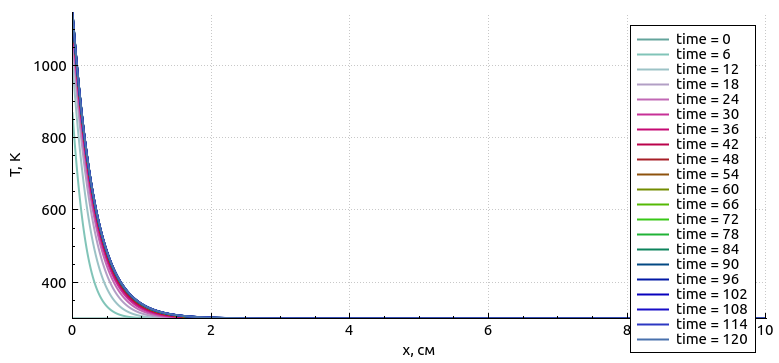
\includegraphics[width=\linewidth]{inc/img/graph1-1}

	На рисунке представлены графики зависимости температуры от координаты при фиксированных $t$ = 0, 6, 12, …


	\item \textbf{График зависимости $T(x_n, t)$ при нескольких фиксированных значениях координаты $x_n$}

	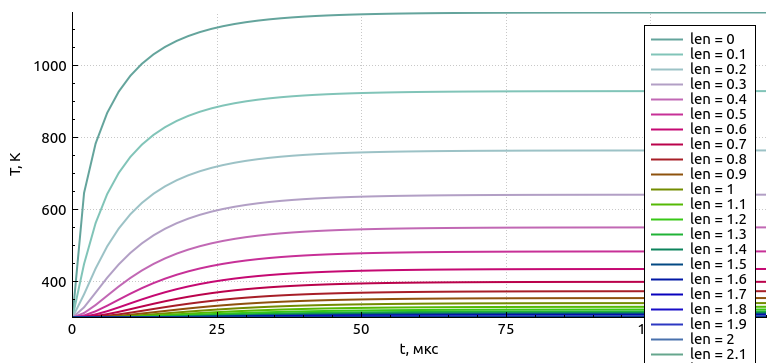
\includegraphics[width=\linewidth]{inc/img/graph1-2}

	На рисунке представлены графики зависимости температуры от времени при фиксированных $x$ = 0, 0.1, 0.2, …, 10.
\end{enumerate}

\section*{Вопросы}

\begin{enumerate}
	\item
	\textbf{
		Приведите результаты тестирования программы (графики, общие соображения, качественный анализ).
		Учесть опыт выполнения лабораторной работы №~3.
	}

	\begin{itemize}
		\item Задать отрицательный тепловой поток.
		Стержень будет охлаждаться с левого торца, а значит $T(x)$ от $0$ до $l$ будет увеличиваться.

		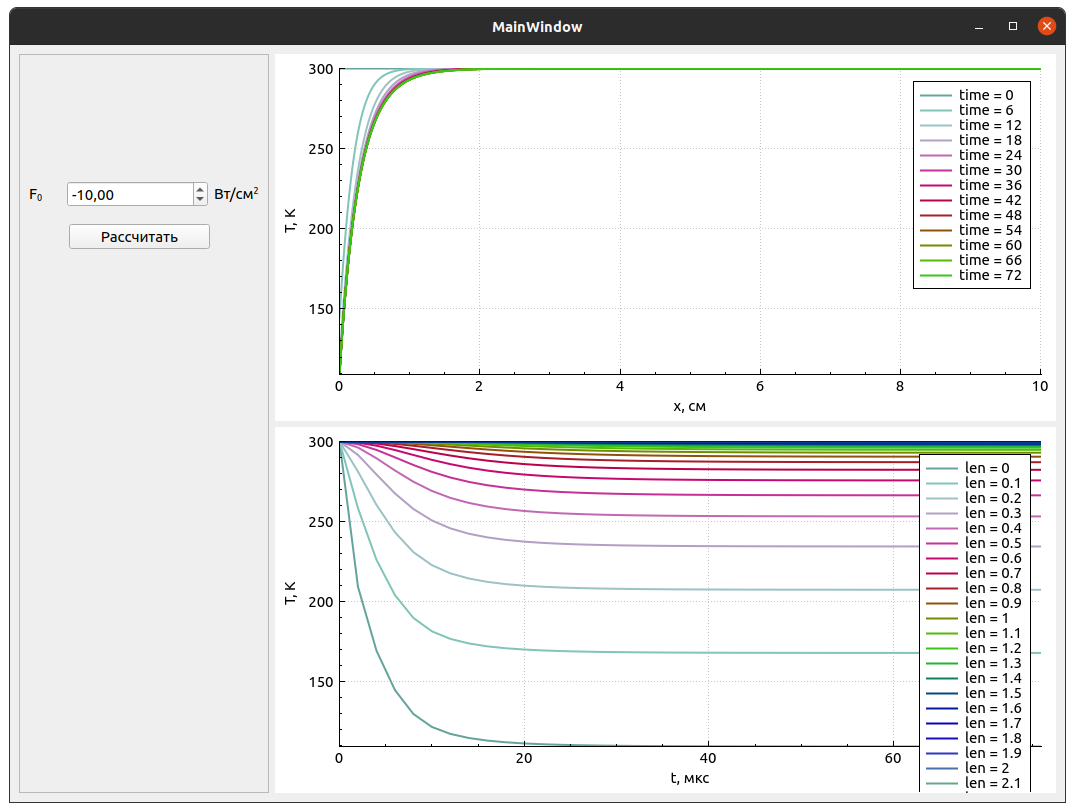
\includegraphics[width=\linewidth]{inc/img/graph3}

		\item При большей теплоотдачи стержня его температура должна снизиться.

		\item При нулевом тепловом потоке температура стержня должна быть неизменной и равняться температуре окружающей среды.

		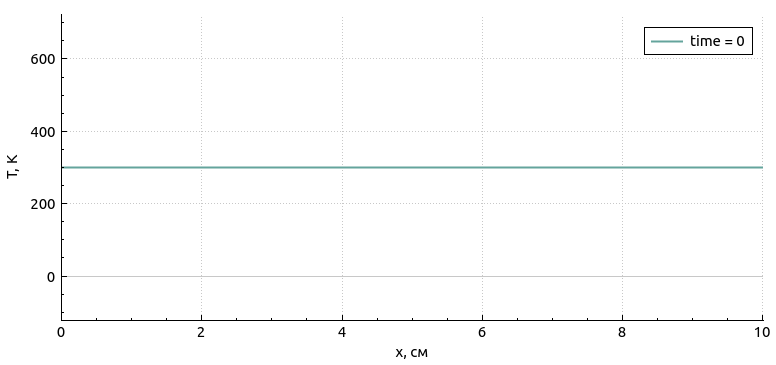
\includegraphics[width=\linewidth]{inc/img/graph2-1}

		\item Свойства материала стержня привязаны к температуре, теплоемкость и коэффициент теплопроводности  зависят от $T$, поменяем зависимости: установим зависимости $T$ от $х$, а $с = 0$.
		Тогда температурное поле $T(x,t)$ должно совпасть с температурным распределением $T(x)$ из лабораторной 3.

		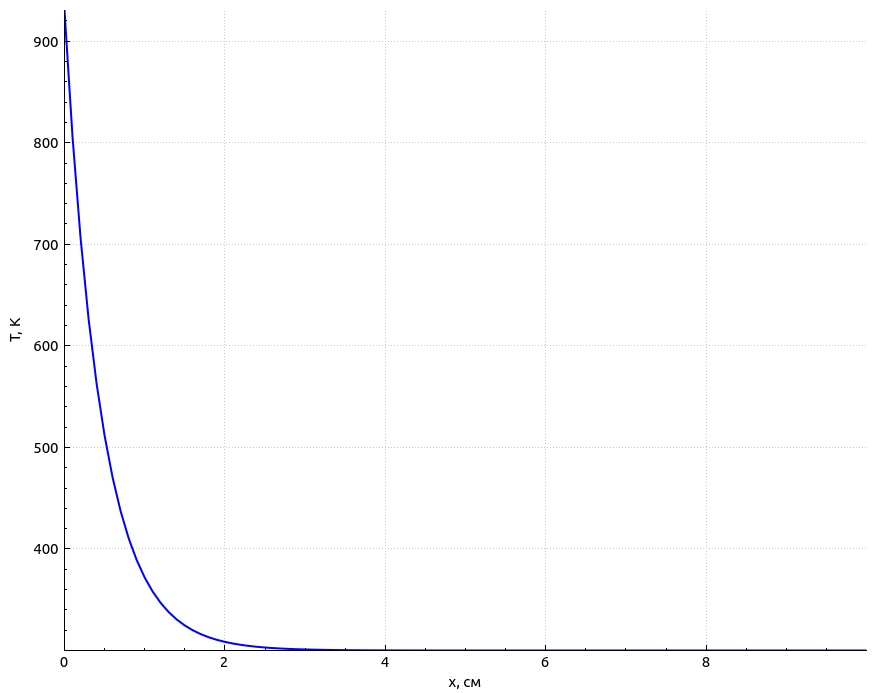
\includegraphics[width=\linewidth]{inc/img/graph4-1}

		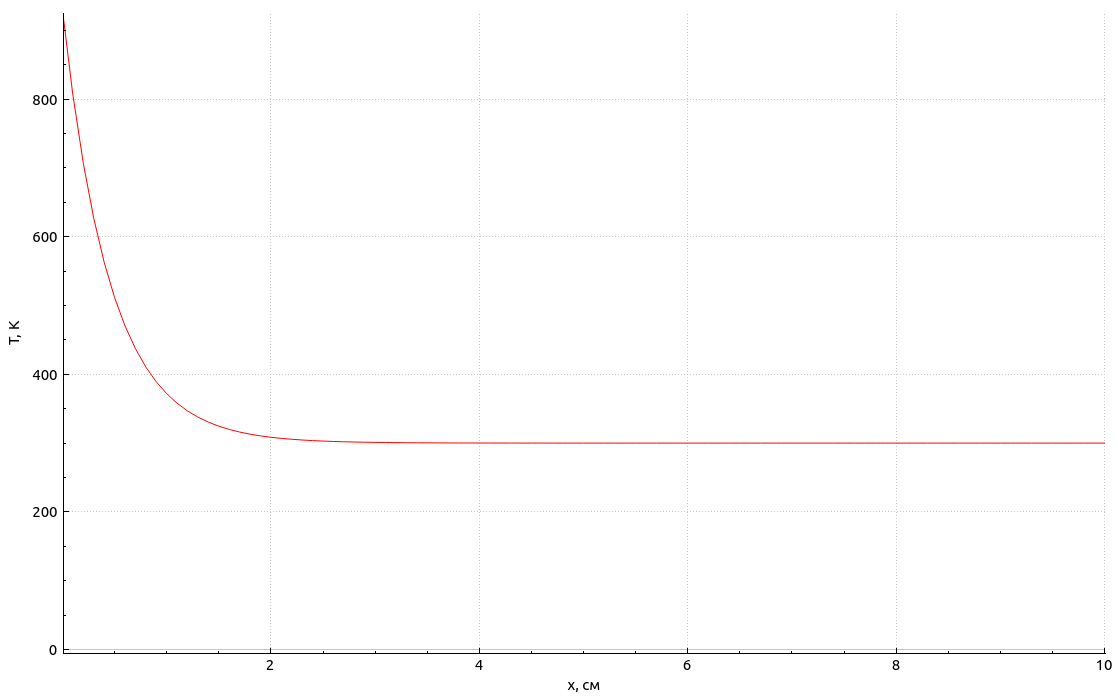
\includegraphics[width=\linewidth]{inc/img/graph4-2}

		На первом рисунке представлен график из 4 работы с изменёнными параметрами, а на втором — из 3.
		Видно, что графики совпадают, пиковые температуры на левых торцах одинаковые, на правых — равны температуре окружающей среды.
		Может показаться, что графики различаются, но это не так.
		Визуальные различия связаны с разным масштабом координатной плоскости.
	\end{itemize}


	\item
	\textbf{
		Выполните линеаризацию уравнения (14.8) по Ньютону, полагая для простоты, что все коэффициенты зависят только от одной переменной $\widehat y_N$.
		Приведите линеаризованный вариант уравнения и опишите алгоритм его решения.
		Воспользуйтесь процедурой вывода, описанной в лекции №~8.
	}

	Система квазилинейных разностных уравнений имеет канонический вид
	\begin{equation*}
		\left\{
		\begin{aligned}
			&\widehat K_0\widehat y_0 + \widehat M_0\widehat y_1 = \widehat P_0,\\
			&\widehat A_n\widehat y_{n-1} - \widehat B_n\widehat y_n + \widehat D_n\widehat y_{n+1}=-\widehat F_n, \quad 1\leqslant n\leqslant N-1,\\
			&\widehat K_N\widehat y_N + \widehat M_N\widehat y_{N-1} = \widehat P_N.\\
		\end{aligned}
		\right.
	\end{equation*}

	Учитывая зависимость только от одной переменной $\widehat y_N$
	\begin{equation*}
		\widehat A_n=\widehat A_n(\widehat y_n),\quad
		\widehat B_n=\widehat B_n(\widehat y_n),\quad
		\widehat D_n=\widehat D_n(\widehat y_n),\quad
		\widehat F_n=\widehat F_n(\widehat y_n),
	\end{equation*}
	выполним линеаризацию по Ньютону
	\begin{multline*}
		\left(\widehat A_n\widehat y_{n-1} - \widehat B_n\widehat y_n + \widehat D_n\widehat y_{n+1} + \widehat F_n\right)\bigg|_{(s-1)}
		+\widehat A_n^{(s-1)}\Delta\widehat y_{n-1}^{(s)}
		+\\+\left(\frac{\partial\widehat A_n}{\partial\widehat y_n}\widehat y_{n-1}-\frac{\partial\widehat B_n}{\partial\widehat y_n}\widehat y_n-\widehat B_n+\frac{\partial\widehat D_n}{\partial\widehat y_n}\widehat y_{n+1}+\frac{\partial\widehat F_n}{\partial\widehat y_n}\right)\bigg|_{(s-1)}
		\cdot\Delta\widehat y_n^{(s)}+\widehat D_n^{(s-1)}\Delta\widehat y_{n+1}^{(s)}
		=0.
	\end{multline*}

	Тогда
	\begin{equation*}
		A_n\Delta\widehat y_{n-1}^{(s)} - B_n\Delta\widehat y_{n}^{(s)} + D_n\Delta\widehat y_{n+1}^{(s)} = -F_n
	\end{equation*}

	\begin{equation*}
		\left\{
		\begin{aligned}
			&A_n=\widehat A_n^{(s-1)},\\
			&B_n=\left(-\frac{\partial\widehat A_n}{\partial\widehat y_n}\widehat y_{n-1} + \frac{\partial\widehat B_n}{\partial\widehat y_n}\widehat y_n + \widehat B_n-\frac{\partial\widehat D_n}{\partial\widehat y_n}\widehat y_{n+1} + \frac{\partial\widehat F_n}{\partial\widehat y_n}\right)\bigg|_{(s-1)},\\
			&D_n=\widehat D_n^{(s-1)},\\
			&F_n=\left(\widehat A_n\widehat y_{n-1}-\widehat B_n\widehat y_n + \widehat D_n\widehat y_{n+1}+\widehat F_n\right)\bigg|_{(s-1)}.
		\end{aligned}
		\right.
	\end{equation*}

	Краевые условия

	\begin{equation*}
		\left\{
		\begin{aligned}
			&\left(\widehat K_0\widehat y_0+\widehat M_0\widehat y_1 - \widehat P_0\right)\bigg|_{(s-1)} + \widehat K_0^{(s-1)}\Delta\widehat y_{0}^{(s)}+\widehat M_0^{(s-1)}\Delta\widehat y_{1}^{(s)}=0,\\
			&\left(\widehat K_N\widehat y_N+\widehat M_N\widehat y_{N-1}- \widehat P_N\right)\bigg|_{(s-1)}+\widehat K_N^{(s-1)}\Delta\widehat y_{N}^{(s)}+\widehat M_N^{(s-1)}\Delta\widehat y_{N-1}^{(s)}=0.
		\end{aligned}
		\right.
	\end{equation*}

	Тогда
	\begin{equation*}
		\left\{
		\begin{aligned}
			&K_0\Delta\widehat y_{0}^{(s)}+M_0\Delta\widehat y_{1}^{(s)}=P_0,\\
			&K_N\Delta\widehat y_{N}^{(s)}+M_N\Delta\widehat y_{N-1}^{(s)}=P_N,\\
		\end{aligned}
		\right.
	\end{equation*}

	\begin{equation*}
		\left\{
		\begin{aligned}
			&K_0=\widehat K_0^{(s-1)},\\
			&M_0=\widehat M_0^{(s-1)},\\
			&P_0=-\left(\widehat K_0 \widehat y_0+ \widehat M_0 \widehat y_1- \widehat P_0\right)\bigg|_{(s-1)},\\
			&K_N=\widehat K_N^{(s-1)},\\
			&M_N=\widehat M_N^{(s-1)},\\
			&P_N=-\left(\widehat K_N \widehat y_N+ \widehat M_N \widehat y_{N-1}-\widehat P_N\right)\bigg|_{(s-1)}.\\
		\end{aligned}
		\right.
	\end{equation*}

	Получаем систему
	\begin{equation}
		\left\{
		\begin{aligned}
			&A_n\Delta\widehat y_{n-1}^{(s)}-B_n\Delta\widehat y_{n}^{(s)}+D_n\Delta\widehat y_{n+1}^{(s)}=-F_n,\\
			&K_0\Delta\widehat y_{0}^{(s)}+M_0\Delta\widehat y_{1}^{(s)}=P_0,\\
			&K_N\Delta\widehat y_{N}^{(s)}+M_N\Delta\widehat y_{N-1}^{(s)}=P_N.\\
		\end{aligned}
		\right.
	\end{equation}

	Решается методом прогонки, в результате находятся все $\Delta \widehat y_n^s$, после чего определяются значения искомой функции в узлах $ \widehat y_n^s= \widehat y_n^{(s-1)}+\Delta \widehat y_n^s $.
	Итерационный процесс заканчивается при выполнении условия $\displaystyle \max\bigg|\frac{\Delta \widehat y_n^s}{\widehat y_n^s}\bigg|\leqslant\varepsilon$.
\end{enumerate}

\pagebreak
\section*{Листинг}

\lstinputlisting[caption={\code{solve.hpp}}, language=C++]{../solve.hpp}

\lstinputlisting[caption={\code{solve.cpp}}, language=C++]{../solve.cpp}

\lstinputlisting[caption={\code{mainwindow.hpp}}, language=C++]{../mainwindow.hpp}

\lstinputlisting[caption={\code{mainwindow.cpp}}, language=C++]{../mainwindow.cpp}

\lstinputlisting[caption={\code{main.cpp}}, language=C++]{../main.cpp}

\lstinputlisting[caption={\code{CMakeLists.txt}}]{../CMakeLists.txt}

\end{document}
